%! TEX root = main.tex

\chapter{Pipes}

This chapter introduces wave propagation in ducts, with emphasis on cylindrical pipes as a model for wind instruments and for air cavities coupled to vibrating structures. The goal is to describe how the acoustic field evolves along the duct, how higher-order modes arise when the cross section cannot be treated as uniform, and how cutoff frequencies determine which modes can effectively propagate. 

\section{Infinite Cylindrical Pipes}

Let us consider an infinite cylindrical pipe deployed along the \( x \) axis, with cross section \( S \). Cylindrical coordinates \( (r,\phi,x) \) are used. We assume rigid, smooth, thermally insulating walls. The basic geometry and notation for an infinite cylindrical duct are summarized in figure \ref{fig:pipe_geometry}.

\begin{figure}[!htb]
    \centering
    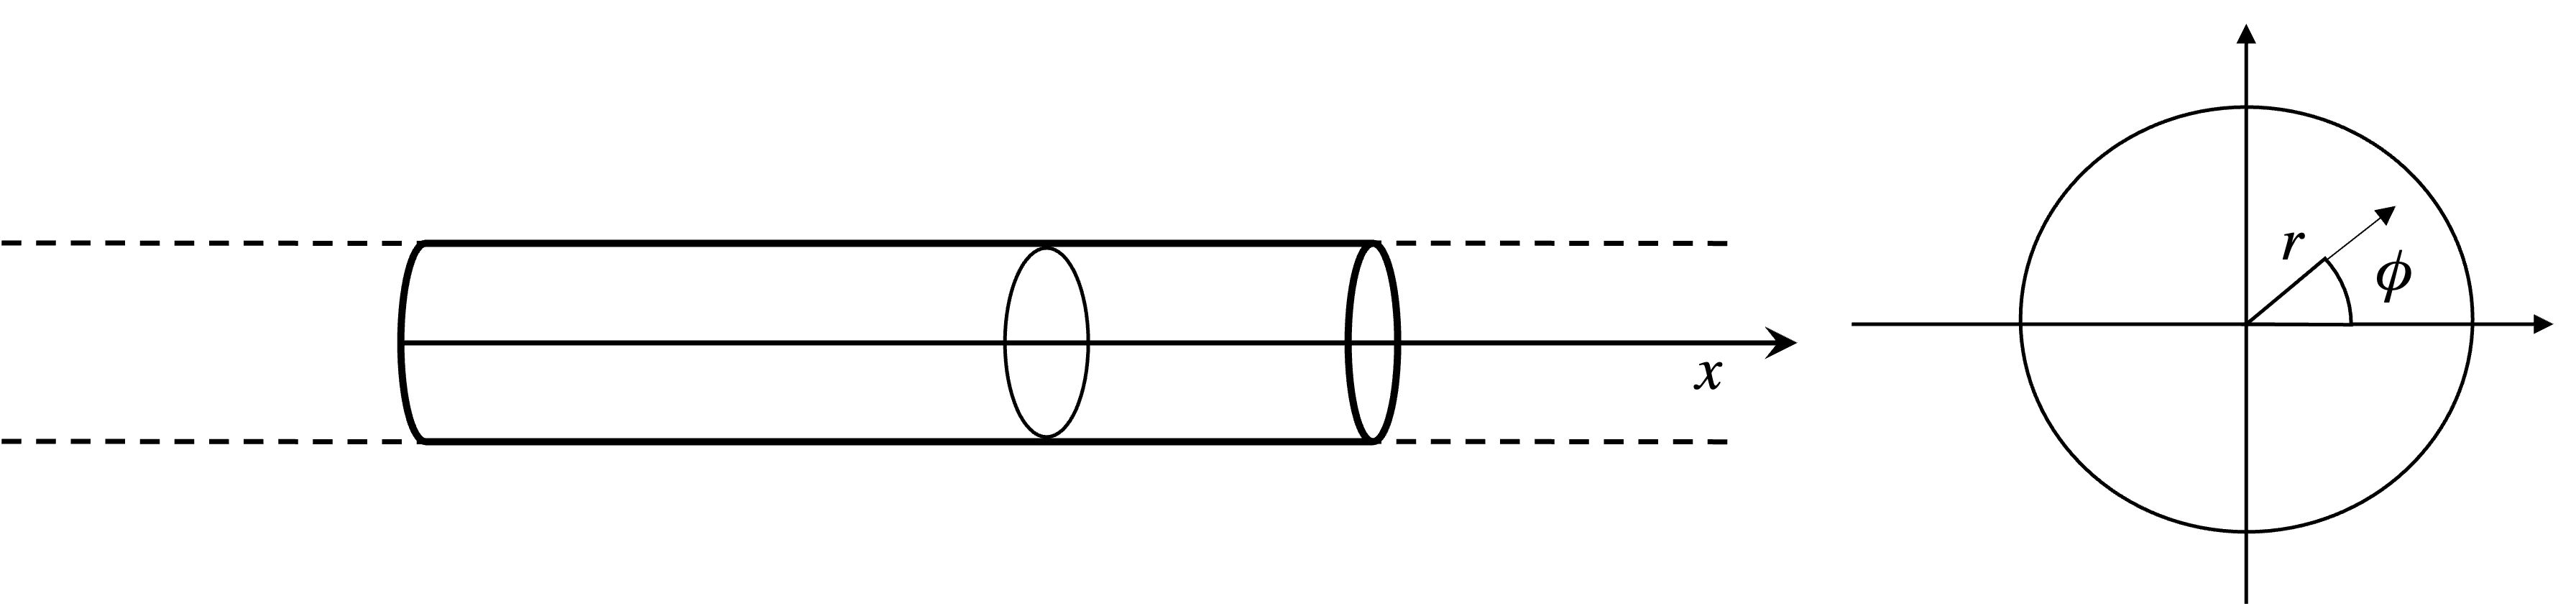
\includegraphics[width=0.60\linewidth]{00_Images/06_chapter/img66.jpg}
    \caption{Geometry of an infinite cylindrical pipe}
    \label{fig:pipe_geometry}
\end{figure}

\subsection{Plane-wave Approximation} 

If the pressure is assumed uniform over the cross section, it depends only on \( x \) and \( t \), and a traveling-wave solution can be written as
\[
p(x,t) = p e^{j(-kx+\omega t)}
\]
The acoustic volume flow is defined as \( U(x,t) \triangleq u(x,t)S \), and under this approximation it becomes
\[
U(x,t) = \frac{S p}{\rho c} e^{j(-kx+\omega t)}
\]
The corresponding characteristic impedance is
\[
Z_{0} = \frac{p(x,t)}{U(x,t)} = \frac{\rho c}{S}
\]
This quantity differs from the wave impedance because the denominator is the volume flow rather than the particle velocity.

\subsection{Wave Equation and Boundary Condition} 

In general, pressure and particle velocity are not uniform over the section, therefore \( p = p(r,\phi,x,t) \). The wave equation in cylindrical coordinates is
\[
\frac{1}{r}\frac{\partial}{\partial r}\left(r\frac{\partial p}{\partial r}\right) + \frac{1}{r^{2}}\frac{\partial^{2}p}{\partial \phi^{2}} + \frac{\partial^{2}p}{\partial x^{2}} = \frac{1}{c^{2}}\frac{\partial^{2}p}{\partial t^{2}}
\]
Let \( a \) be the pipe radius. Rigid walls imply that the radial component of particle velocity vanishes at \( r=a \),
\[
\left.u_{r}(r,\phi,x,t)\right|_{r=a} = 0
\]
Using the linear momentum equation
\[
\rho \frac{\partial \mathbf{u}}{\partial t} = -\nabla p
\]
this condition is equivalent to
\[
\left.\frac{\partial p}{\partial r}\right|_{r=a} = 0
\]

\subsection{Modal Solutions and Cutoff} 

\begin{figure}[!htb]
    \centering
    \subfloat[Pressure and transverse flow patterns]{%
        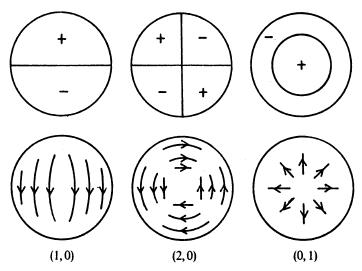
\includegraphics[width=0.4\linewidth]{00_Images/06_chapter/img92.jpg}%
    }\hfill
    \subfloat[Particle-velocity patterns (below cutoff)]{%
        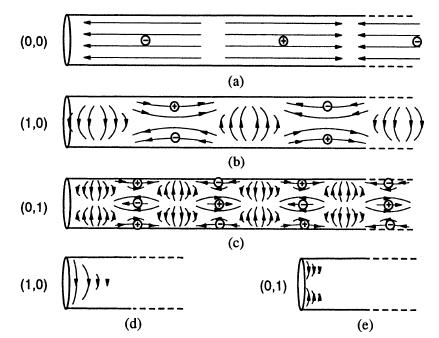
\includegraphics[width=0.4\linewidth]{00_Images/06_chapter/img107.jpg}%
    }
    \caption{Examples of higher-order modal field patterns in a cylindrical duct}
    \label{fig:higher_modes_patterns}
\end{figure}

After separation of variables, the \( (m,n) \) mode propagating in the tube can be written as
\[
p_{mn}(r,\phi,x,t) = p J_{m}\left(\frac{\pi q_{mn} r}{a}\right)
\begin{cases}
\cos(m\phi) \\
\sin(m\phi)
\end{cases}
e^{-jk_{mn}x}e^{j\omega t}
\]
where \( J_{m} \) is the Bessel function of order \( m \). The boundary condition \( \partial p/\partial r|_{r=a}=0 \) requires
\[
J_{m}'(\pi q_{mn}) = 0
\]
therefore \( \pi q_{mn} \) must coincide with a zero of \( J_{m}' \). The axial wavenumber satisfies
\[
k_{mn}^{2} = \left(\frac{\omega}{c}\right)^{2} - \left(\frac{\pi q_{mn}}{a}\right)^{2}
\]
A mode propagates without radial attenuation only if \( k_{mn} \) is real, which defines the cutoff frequency
\[
\omega_{c} = \frac{\pi q_{mn} c}{a}
\]
Below cutoff, the mode becomes evanescent and is strongly attenuated along the duct. The only exception is the \( (0,0) \) mode, for which \( q_{00}=0 \), corresponding to the plane wave that propagates at all frequencies. The index \( m = 0,1,2,\dots \) represents the number of nodal diameters, while \( n = 0,1,2,\dots \) represents the number of nodal circles in the cross section. The transverse structure of higher-order duct modes is illustrated in figure \ref{fig:higher_modes_patterns}.

\section{Wall Losses}

In the ideal plane-wave approximation for the \( (0,0) \) mode, both the axial particle velocity \( u_{x} \) and the pressure \( p \) are assumed uniform over the pipe cross section. In practice, measurements show that they are maximum along the pipe axis and decrease towards the walls. This deviation is due to wall losses, mainly caused by viscous drag and thermal exchange with the pipe boundaries.

\subsection{Viscous Losses} 

Viscous drag exerted by the walls reduces the particle velocity close to the boundary. Wall losses can be interpreted through the development of a viscous boundary layer near the duct wall, as shown in figure \ref{fig:boundary_layer}.

\begin{figure}[!htb]
    \centering
    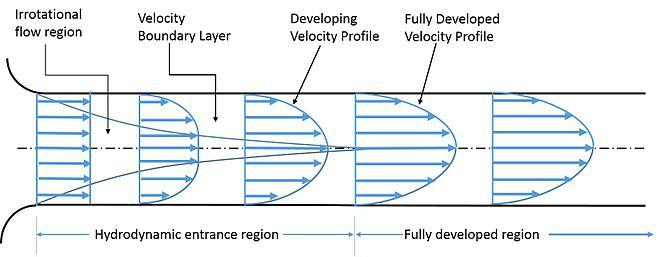
\includegraphics[width=0.75\linewidth]{00_Images/06_chapter/img117.jpg}
    \caption{Development of the viscous boundary layer in the plane-wave mode}
    \label{fig:boundary_layer}
\end{figure}

The region over which this effect is significant is referred to as the viscous boundary layer. Its relevance can be quantified by comparing its thickness to the pipe radius through the dimensionless ratio \( r_{v} \). A commonly used expression is
\[
r_{v} = 632.8 a f^{1/2}(1 - 0.0029\Delta T)
\]
where \( a \) is the pipe radius, \( f \) is the frequency, and \( \Delta T = T - \SI{300}{\kelvin} \). Viscous losses are therefore more important for small pipes.

\subsection{Thermal Losses} 
A similar mechanism arises from heat exchange between air and the walls. The resulting thermal boundary layer modifies the effective compressibility of the air close to the boundary. The associated ratio is
\[
r_{t} = 532.8 a f^{1/2}(1 - 0.0031\Delta T)
\]
with the same definitions as above. 

\subsection{Consequences on Propagation} 

The combined effect of viscous and thermal losses makes the characteristic impedance \( Z_{0} \) complex and different from \( \rho c/S \), and the wavenumber becomes complex as well, leading to attenuation along the duct. Writing
\[
k = \frac{\omega}{v} - j\alpha
\]
the phase velocity \( v \) and the attenuation coefficient \( \alpha \) can be described as functions of \( r_{v} \). For sufficiently large tubes, approximate expressions valid for \( r_{v} > 10 \) are
\[
v \approx c\left[1 - \frac{1.65 \times 10^{-3}}{a f^{1/2}}\right]
\]
\[
\alpha \approx \frac{3 \times 10^{-5} f^{1/2}}{a}
\]
The trends are summarized in the plots of the real and imaginary parts of \( Z_{0} \) as functions of \( r_{v} \), and of \( v/c \) and \( \alpha/f \) versus \( r_{v} \). The influence of viscous and thermal losses on the characteristic impedance is summarized in figure \ref{fig:char_impedance_parts} and the corresponding effects on phase speed and attenuation are illustrated in figure \ref{fig:phase_speed_attenuation}.

\begin{figure}[!htb]
    \centering
    \subfloat{%
        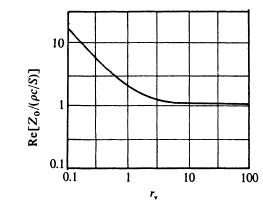
\includegraphics[width=0.4\linewidth]{00_Images/06_chapter/img148.jpg}%
    }\hfill
    \subfloat{%
        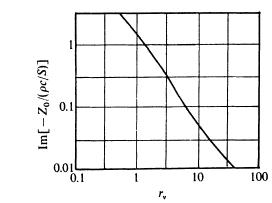
\includegraphics[width=0.4\linewidth]{00_Images/06_chapter/img158.jpg}%
    }
    \caption{Real and imaginary parts of the characteristic impedance versus the loss parameter}
    \label{fig:char_impedance_parts}
\end{figure} 

\begin{figure}[!htb]
    \centering
    \subfloat{%
        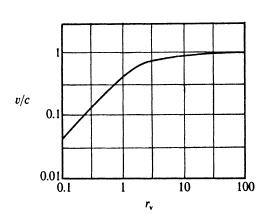
\includegraphics[width=0.4\linewidth]{00_Images/06_chapter/img206.jpg}%
    }\hfill
    \subfloat{%
        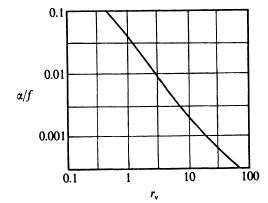
\includegraphics[width=0.4\linewidth]{00_Images/06_chapter/img216.jpg}%
    }
    \caption{Phase speed and attenuation coefficient in a lossy cylindrical duct}
    \label{fig:phase_speed_attenuation}
\end{figure}

\section{Finite Cylindrical Pipes}

From now on we assume that only the plane mode \( m = 0 \), \( n = 0 \) is present, so that pressure and volume flow depend on \( x \) and \( t \) only. The pressure field is written as the superposition of two counter-propagating waves
\[
p(x,t) = \left[Ae^{-jkx} + Be^{jkx}\right]e^{j\omega t}
\]
Using \( \rho \partial u/\partial t = -\nabla p \), the acoustic volume flow \( U(x,t) = Su(x,t) \) becomes
\[
U(x,t) = \frac{S}{\rho c}\left[Ae^{-jkx} - Be^{jkx}\right]e^{j\omega t}
\]
where \( S \) is the cross-sectional area and \( Z_{0} = \rho c/S \) is the characteristic impedance of the duct.

\subsection{Termination and Input Impedance}

Let the duct be terminated at \( x=L \) by a load impedance \( Z_{L} \), defined by
\[
\frac{p(L,t)}{U(L,t)} = Z_{L}
\]
Imposing the termination condition yields ratio between backward and forward waves
\[
\frac{B}{A} = e^{-2jkL}\left(\frac{Z_{L} - Z_{0}}{Z_{L} + Z_{0}}\right)
\]
The input impedance, defined at \( x=0 \) as \( Z_{\mathrm{IN}} = p(0,t)/U(0,t) \), is
\[
Z_{\mathrm{IN}} = Z_{0}\left[\frac{Z_{L}\cos(kL) + jZ_{0}\sin(kL)}{jZ_{L}\sin(kL) + Z_{0}\cos(kL)}\right]
\]

\begin{figure}[!htb]
    \centering
    \subfloat[Stopped End]{%
        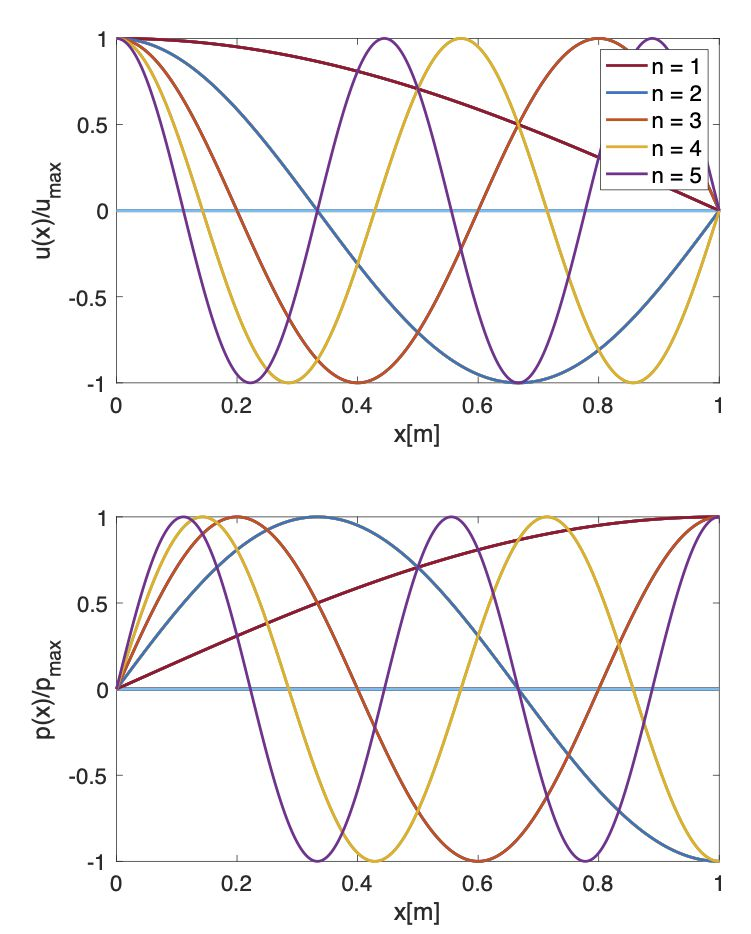
\includegraphics[height=0.4\textheight]{00_Images/06_chapter/img230.jpg}%
    }\hfill
    \subfloat[Open End]{%
        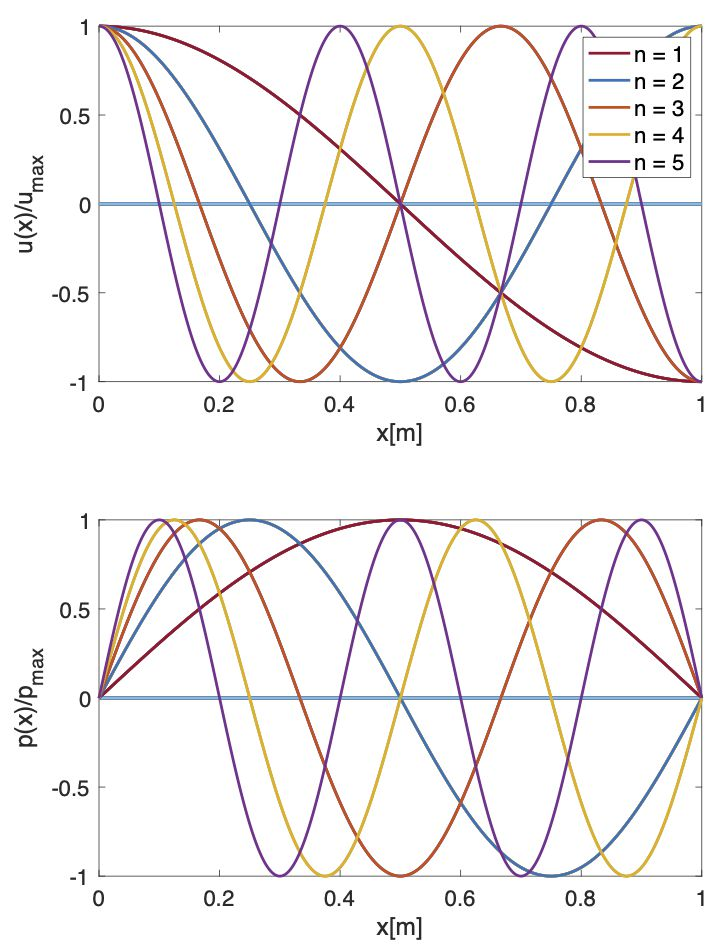
\includegraphics[height=0.4\textheight]{00_Images/06_chapter/img241.jpg}%
    }
    \caption{Examples of pressure and velocity distributions in finite pipes}
    \label{fig:finite_pipe_fields}
\end{figure}

\subsection{Stopped End}

For a stopped termination \( Z_{L} \to \infty \), the input impedance reduces to
\[
Z_{\mathrm{IN}}^{\mathrm{stopped}} = -jZ_{0}\cot(kL)
\]
Impedance minima occur at
\[
\omega_{\mathrm{stopped}} = \frac{(2n-1)\pi c}{2L}
\]
which corresponds to an odd number of quarter wavelengths in the pipe. 

\subsection{Open End and Radiation Load}

For an ideal open termination \( Z_{L} = 0 \),
\[
Z_{\mathrm{IN}}^{\mathrm{open}} = jZ_{0}\tan(kL)
\]
and for \( kL \ll 1 \),
\[
Z_{\mathrm{IN}}^{\mathrm{open}} \approx jZ_{0}kL
\]
The corresponding impedance minima occur at
\[
\omega_{\mathrm{open}} = \frac{n\pi c}{L}
\]
which corresponds to an even number of quarter wavelengths. In practice, a truly open end implies radiation outside the duct, therefore the termination cannot be modeled with \( p(L,t)=0 \) and a radiation load must be introduced.

\subsection{End Correction}

If the pipe terminates in a plane flange, the radiation load can be written as \( Z_{\mathrm{flanged}} = R + jX \) with
\[
R = Z_{0}\left[\frac{(ka)^{2}}{2} - \frac{(ka)^{4}}{2^{2}\cdot 3} + \frac{(ka)^{6}}{2^{2}\cdot 3^{2}\cdot 4} - \dots\right]
\]
\[
X = \frac{Z_{0}}{\pi k^{2}a^{2}}\left[\frac{(2ka)^{3}}{3} - \frac{(2ka)^{5}}{3^{2}\cdot 5} + \frac{(2ka)^{7}}{3^{2}\cdot 5^{2}\cdot 7} - \dots\right]
\]
In the region \( ka \ll 1 \), the impedance is approximately reactive
\[
Z_{\mathrm{flanged}} \approx jZ_{0}k\left(\frac{8a}{3\pi}\right)
\]
Since a short open pipe segment of length \( \Delta \) has \( Z_{\mathrm{IN}} \approx jZ_{0}k\Delta \) for \( k\Delta \ll 1 \), the radiation load can be assimilated to a virtual elongation
\[
\Delta_{\mathrm{flanged}} = \frac{8a}{3\pi} \approx 0.85a
\]
Therefore a real open pipe can be approximated as an ideal open pipe of effective length \( L + \Delta_{\mathrm{flanged}} \), so that radiation is included through an end correction. For an unflanged pipe, a commonly used low-frequency approximation is
\[
\Delta_{\mathrm{unflanged}} \approx 0.6a
\]
The end-correction model can be extended with reasonable accuracy up to \( ka = 3 \). For \( ka > 3 \), radiation losses become significant and the load cannot be treated as purely reactive, so the simple virtual-elongation picture is no longer sufficient. The frequency dependence of the end correction is shown in figure \ref{fig:end_correction}.

\begin{figure}[!htb]
    \centering
    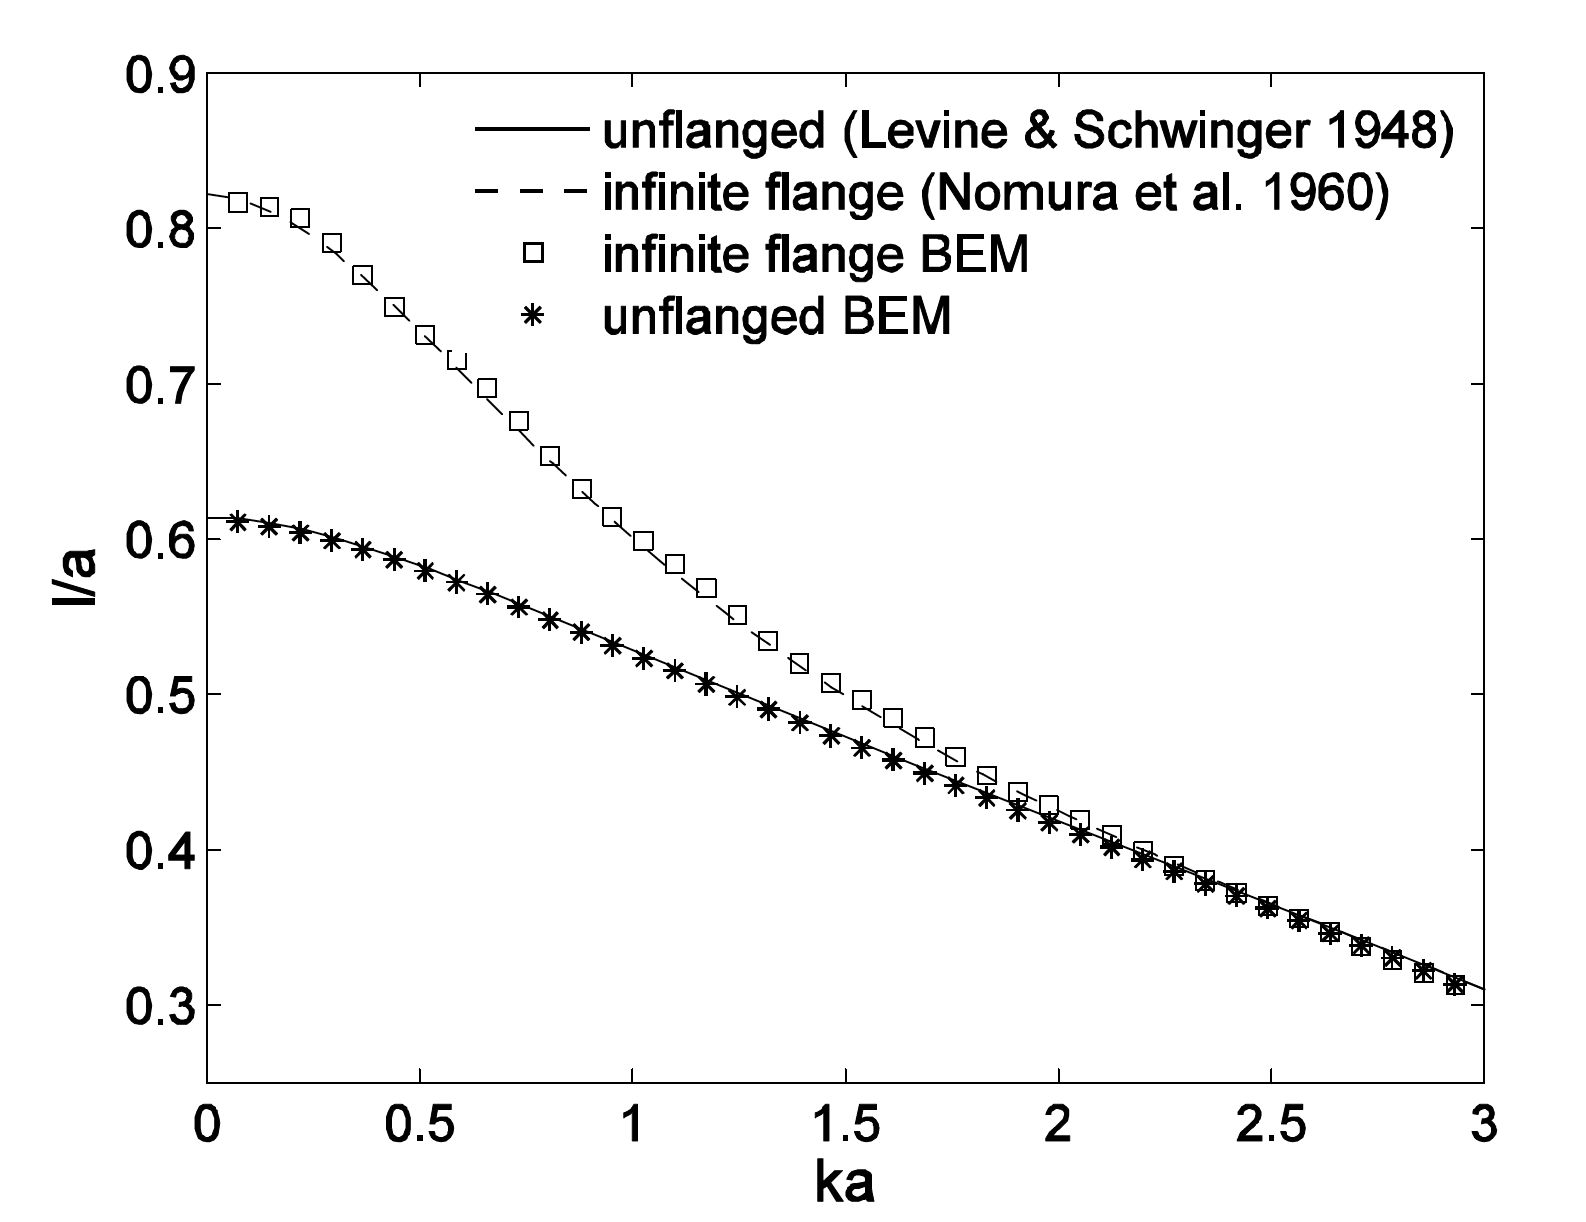
\includegraphics[width=0.80\linewidth]{00_Images/06_chapter/img265.jpg}
    \caption{Normalized end correction for flanged and unflanged terminations}
    \label{fig:end_correction}
\end{figure}


\subsection{Directional Properties and Directivity Index}

The directional properties of the radiation can be described through the angular distribution of intensity. The radiated intensity at angle \( \theta \) is proportional to
\[
\left[\frac{2J_{1}(ka\sin\theta)}{ka\sin\theta}\right]^{2}
\]
where \( J_{1} \) is the Bessel function of first order. A compact summary of directionality is provided by the directivity index \( DI \), defined as the sound intensity on the axis compared with that of an isotropic source radiating the same total radiated power. The transition from nearly omnidirectional radiation to more directional patterns with increasing \( ka \) is illustrated in figure \ref{fig:pipe_directivity}.

\begin{figure}[!htb]
    \centering
    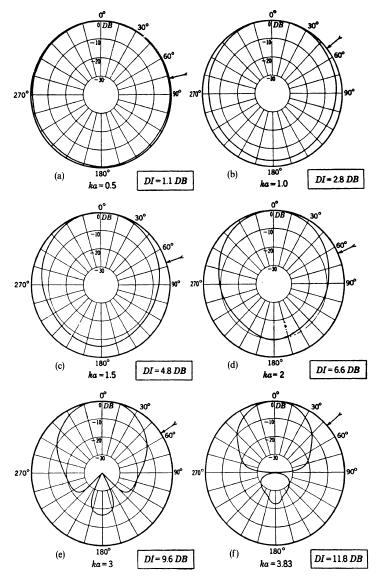
\includegraphics[width=0.60\linewidth]{00_Images/06_chapter/img282.jpg}
    \caption{Radiation directivity of a circular pipe opening for increasing \(ka\)}
    \label{fig:pipe_directivity}
\end{figure}

\section{Impedance Curves}

Including wall losses leads to a complex wavenumber
\[
k = \frac{\omega}{v} - j\alpha
\]
where \( v \) is the phase velocity and \( \alpha \) is the attenuation coefficient. As a consequence, the input impedance of a finite pipe can be expressed in terms of hyperbolic functions. For an open pipe, a convenient form is
\[
Z_{\mathrm{IN}} = Z_{0}\left[\frac{\tanh(\alpha L) + j\tan(\omega L/v)}{1 + j\tanh(\alpha L)\tan(\omega L/v)}\right]
\]
The auxiliary functions \( \tanh(\cdot) \) and \( \coth(\cdot) \) are often used to describe how the resonance peaks are affected by losses. 

\subsection{Maxima and Minima}

Wall losses do not modify the location of maxima and minima with respect to the ideal lossless case, but they strongly affect their magnitude. In particular, the impedance magnitude at resonance maxima is
\[
|Z_{\mathrm{IN}}|_{\max} = Z_{0}\coth(\alpha L)
\]
while at the minima it is
\[
|Z_{\mathrm{IN}}|_{\min} = Z_{0}\tanh(\alpha L)
\]
Since \( \alpha \) increases with frequency, the maxima of \( Z_{\mathrm{IN}} \) progressively converge to \( Z_{0} \) at high frequencies.

\subsection{Role of Pipe Size}

The relative importance of the different loss mechanisms depends on the pipe radius. In narrow pipes, wall losses dominate already at low frequencies. In wide pipes, wall losses are weaker and radiation losses from the open end become more important at high frequencies. This behavior is reflected by the impedance curves shown for a pipe of length \SI{1}{\metre} with radius \SI{2}{\centi\metre} and \SI{10}{\centi\metre}, where the peak magnitudes evolve differently with frequency. The effect of duct radius on the input impedance in the presence of losses is illustrated in figure \ref{fig:wide_narrow_impedance}.

\begin{figure}[!htb]
    \centering
    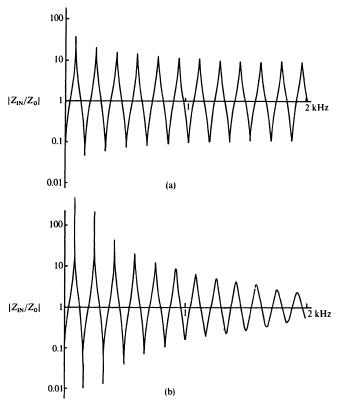
\includegraphics[width=0.60\linewidth]{00_Images/06_chapter/img327.jpg}
    \caption{Input impedance comparison for wide and narrow cylindrical pipes}
    \label{fig:wide_narrow_impedance}
\end{figure}

\section{Horns}

In horns the cross section varies along the axis, therefore the planar-wave assumption becomes less accurate. A useful approximation can be obtained when the horn does not flare too rapidly. In this case, wavefronts can be treated as spherical and orthogonal to the horn walls. The wavefront can be represented as a spherical cap of area \( S \) with curvature radius \( r \), and an equivalent circular cross section of radius \( a \). The geometrical interpretation is summarized in figure \ref{fig:webster_geometry}.

\begin{figure}[!htb]
    \centering
    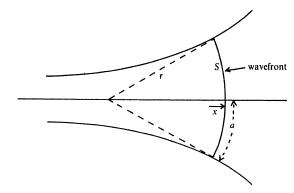
\includegraphics[width=0.45\linewidth]{00_Images/06_chapter/img343.jpg}
    \caption{Wavefront geometry and cross-sectional area \(S(x)\) in a horn}
    \label{fig:webster_geometry}
\end{figure}

\subsection{Horn Wave Equation and Propagation Condition}

Let \( x \) be the coordinate along the horn axis. Due to the progressive increase of the cross section, the pressure amplitude decreases with \( x \). It is convenient to introduce
\[
\psi = p S^{-1/2}
\]
For a circular horn, \( \psi \) satisfies
\[
\frac{\partial^{2}\psi}{\partial x^{2}} + \left(k^{2} - \frac{1}{a}\frac{\partial^{2}a}{\partial x^{2}}\right)\psi = 0
\]
with \( k = \omega/c \). The quantity
\[
F = \frac{1}{a}\frac{\partial^{2}a}{\partial x^{2}}
\]
is the barrier function of the horn. The solution corresponds to a propagating wave if
\[
k^{2} - F > 0
\]
therefore frequencies such that \( k^{2} > F \) can propagate, whereas frequencies such that \( k^{2} < F \) do not propagate.

\subsection{Slowly Flaring Horns}

For horns that do not flare too rapidly, \( F \) can be approximated as
\[
F \approx \frac{1}{R_{L}R_{T}}
\]
where \( R_{L} \) is the longitudinal radius of curvature and \( R_{T} \) is the internal transverse radius of curvature. This two radii of curvature are defined in figure \ref{fig:curvature_radii}.

\begin{figure}[!htb]
    \centering
    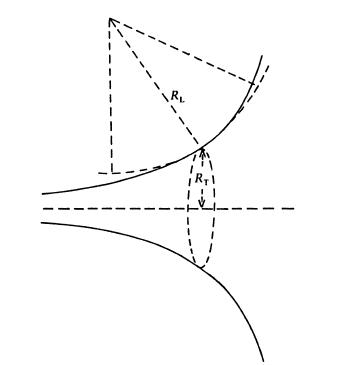
\includegraphics[width=0.45\linewidth]{00_Images/06_chapter/img359.jpg}
    \caption{Definition of longitudinal and transverse curvature radii \(R_L\) and \(R_T\)}
    \label{fig:curvature_radii}
\end{figure}

\subsection{Salmon Horns}

In Salmon horns the barrier function \( F \) is constant along the axis, hence the cutoff frequency is constant throughout the horn. An equivalent radius can be written as
\[
a = a_{0}\left[\cosh(mx) + T\sinh(mx)\right]
\]
A corresponding pressure wave is
\[
p = \left(\frac{p_{0}}{a}\right)e^{j\omega t}e^{-j\sqrt{k^{2}-m^{2}}x}
\]
and it does not propagate if \( k < m \). Different horn profiles are obtained by varying \( T \). 

\paragraph{Exponential horn} If \( T = 1 \),
\[
a = a_{0}e^{mx}
\]

\paragraph{Catenoidal horn} If \( T = 0 \),
\[
a = a_{0}\cosh(mx)
\]
This profile smoothly joins a cylindrical pipe extending along the negative axis to the origin.

\paragraph{Conical horn} If \( T = 1/(mx_{0}) \) and \( m \to 0 \),
\[
a = a_{0}\left(1 + \frac{x}{x_{0}}\right)
\]
The vertex is at \( -x_{0} \) and the semiangle is \( \tan^{-1}(a_{0}/x_{0}) \). In this case \( F = 0 \), therefore the conical horn has no cutoff.

\section{Finite Conical and Bessel Horns}

In practical instruments horns have finite length and are connected to the rest of the duct by a throat section. The input impedance must therefore account for the termination at the mouth and for the geometric parameters of the profile. 

\subsection{Finite Conical and Exponential Horns}

Consider a conical horn with throat area \( S_{1} \) at position \( x_{1} \) and mouth area \( S_{2} \) at position \( x_{2} \), with \( L = x_{2} - x_{1} \). If the horn is terminated by a load impedance \( Z_{L} \) at the mouth, the input impedance at the throat can be written as
\[
Z_{\mathrm{IN}} = \frac{\rho c}{S_{1}}
\frac{
jZ_{L}\left[\sin(kL-\theta_{2})/\sin\theta_{2}\right] + (\rho c/S_{2})\sin kL
}{
Z_{L}\left[\sin(kL+\theta_{1}-\theta_{2})/(\sin\theta_{1}\sin\theta_{2})\right] - (j\rho c/S_{2})\left[\sin(kL+\theta_{1})/\sin\theta_{1}\right]
}
\]
where the angles \( \theta_{1} \) and \( \theta_{2} \) depend on the distance from the cone apex. In particular, defining \( x_{1/2} \) as the distance from the apex,
\[
\theta_{1}/2 = \tan^{-1}(kx_{1/2})
\]
For an exponential horn of length \( L \), the input impedance can be expressed as
\[
Z_{\mathrm{IN}} = \frac{\rho c}{S_{1}}
\frac{
Z_{L}\cos(bL+\theta) + j(\rho c/S_{2})\sin bL
}{
jZ_{L}\sin bL + (\rho c/S_{2})\cos(bL-\theta)
}
\]
with
\[
b^{2} = k^{2} - m^{2}
\]
and
\[
\theta = \tan^{-1}(m/b)
\]
A representative magnitude of the input impedance for a conical horn is shown in figure \ref{fig:conical_horn_impedance}.

\begin{figure}[!htb]
    \centering
    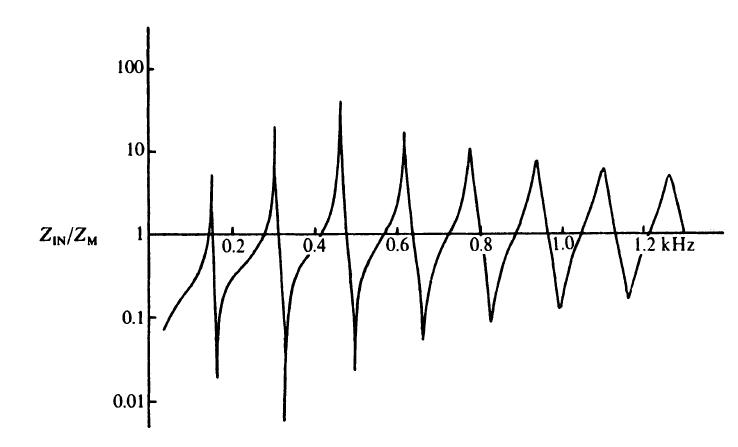
\includegraphics[width=0.7\linewidth]{00_Images/06_chapter/img375.jpg}
    \caption{Magnitude of the input impedance of a conical horn}
    \label{fig:conical_horn_impedance}
\end{figure}

\subsection{Conical Horns}

For an open conical horn, \( Z_{L} = 0 \), and the previous expression reduces to
\[
Z_{\mathrm{IN}} = j\left(\frac{\rho c}{S_{1}}\right)\frac{\sin kL \sin\theta_{1}}{\sin(kL+\theta_{1})}
\]
Zeros occur when \( \sin kL = 0 \), hence at the same frequencies as an open cylindrical pipe of length \( L \). Maxima occur when the denominator vanishes, which can be written as
\[
kL = n\pi - \tan^{-1}(kx_{1})
\]
The impedance magnitude therefore exhibits a sequence of peaks whose spacing remains essentially harmonic, while their heights decrease as frequency increases, consistently with the trend shown by the normalized impedance plot for a \SI{1}{\metre} horn. 

\subsection{Bessel Horns and Rapidly Flaring Profiles}

A broader class of horn profiles is described by Bessel horns, defined by
\[
S = Bx^{-2\epsilon}
\]
and
\[
a = bx^{-\epsilon}
\]
where \( x \) is the distance from a reference point \( x=0 \). When \( \epsilon > 0 \), the horn flares rapidly. For rapidly flaring horns it is important to interpret the barrier function with care. For exponential horns, a plane-wave based description predicts that the barrier function becomes unbounded as \( x \to 0 \), which would imply no propagation in that region. An example of Bessel-horn profile is shown in figure \ref{fig:bessel_horn_shape}. However, the plane-wave approximation is not applicable when the flare is rapid. Close to the open end, a spherical-wave description is more appropriate and leads to a different effective barrier function, as illustrated by the comparison between plane-wave and spherical-wave horn functions. The horn function and the accuracy of common approximations are compared in figure \ref{fig:horn_function_F}.

\begin{figure}[!htb]
    \centering
    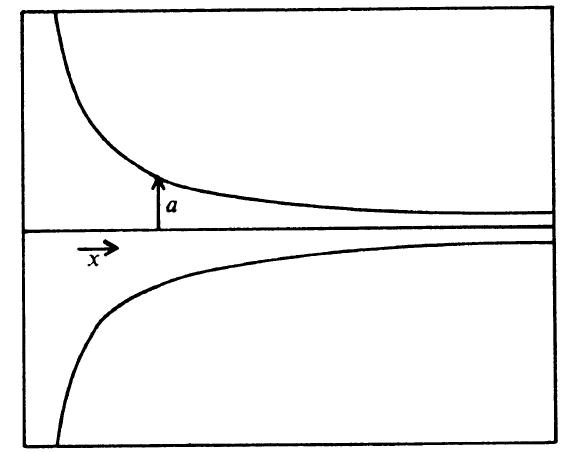
\includegraphics[width=0.50\linewidth]{00_Images/06_chapter/img391.jpg}
    \caption{Example geometry of a Bessel horn}
    \label{fig:bessel_horn_shape}
\end{figure}

\begin{figure}[!htb]
    \centering
    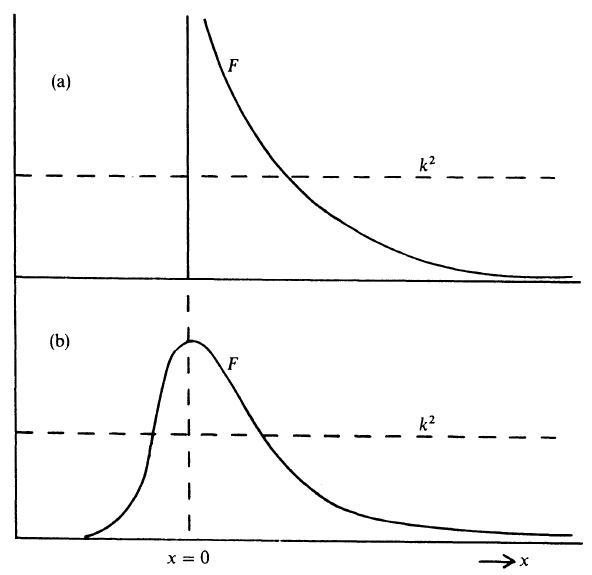
\includegraphics[width=0.60\linewidth]{00_Images/06_chapter/img407.jpg}
    \caption{Horn function \(F\) for Bessel cones: plane-wave and spherical-wave approximations}
    \label{fig:horn_function_F}
\end{figure}

\section{Compound Horns}

Most brass instruments are based on the combination of different duct profiles, rather than on a single uniform geometry. A typical configuration consists of a section with constant cross section followed by an expanding section. Two common examples are a conical horn smoothly joined to a cylindrical section, which is representative of older instruments, and a conical horn smoothly joined to an exponential section, which is representative of modern designs. 

\subsection{Cylindrical Throat Coupled to a Conical Mouth}

Let us consider a cylindrical section of length \( L_{2} \) connected to a conical section of length \( L_{1} \). The overall input impedance is obtained by using, as terminating impedance of the cylindrical section, the input impedance of the conical one. The input impedance of the conical section, evaluated at the junction with area \( S_{1} \), is
\[
Z_{c} = \frac{j\rho c}{S_{1}}\left(\cot kL_{1} + \frac{1}{kx_{1}}\right)^{-1}
\]
where \( x_{1} \) is the distance from the cone apex to the junction. This impedance plays the role of load \( Z_{L} \) for the cylindrical throat. Replacing \( Z_{L} = Z_{c} \) into the expression of the input impedance of the cylindrical section yields a condition for the maxima of the global input impedance. These maxima are found where
\[
\tan kL_{2} - \cot kL_{1} - \left(\frac{1}{kx_{1}}\right) = 0
\]
The resulting peak pattern depends on the relative lengths \( L_{1} \) and \( L_{2} \), as illustrated by the impedance-maxima plot for the compound geometry. The relation between horn shape and the positions of impedance maxima is illustrated in figure \ref{fig:compound_horn_maxima}.

\begin{figure}[!htb]
    \centering
    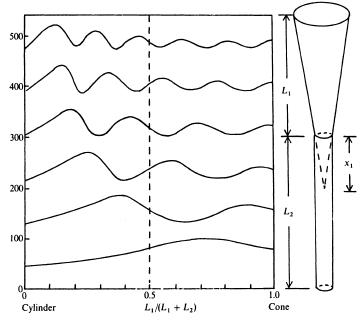
\includegraphics[width=0.55\linewidth]{00_Images/06_chapter/img423.jpg}
    \caption{Maxima of input impedance for a compound horn profile}
    \label{fig:compound_horn_maxima}
\end{figure}

\subsection{Cylindrical Throat Coupled to an Exponential Mouth}

A similar procedure applies when the cylindrical section is connected to an exponential horn. In that case, the condition for the maxima of the global input impedance can be written as
\[
\tan kL_{2} - \frac{b}{k}\cot bL_{1} - \frac{m}{k} = 0
\]
where
\[
b = (k^{2} - m^{2})^{1/2}
\]
and \( m \) is the exponential flare parameter. 

\section{Perturbations}

In real wind instruments the duct geometry is rarely smooth and uniform. Local irregularities, such as fingerholes or small changes in cross section, introduce perturbations that modify the resonance frequencies. These effects can be exploited to tune the instrument response and to obtain a desired harmonic structure. Let the nominal section be \( S_{0}(x) \) and introduce a small perturbation \( \delta S(x) \), so that
\[
S(x) = S_{0}(x) + \delta S(x)
\]
The corresponding pressure distribution is written as
\[
p(x,t) = \beta p_{0}(x,t) + p_{1}(x,t)
\]
where \( p_{0} \) is the unperturbed solution and \( \beta \approx 1 \) under the assumption of a small perturbation. The perturbed resonance frequency is
\[
\omega = \omega_{0} + \delta\omega
\]
By substituting these expressions into the wave equation, retaining first-order terms, and integrating over the horn length, the resonance shift can be written as
\[
\delta\omega
=
-\frac{c^{2}}{2\omega_{0}N}
\int S_{0}\frac{d}{dx}\left(\frac{\delta S}{S_{0}}p_{0}\frac{dp_{0}}{dx}\right)dx
\]
where
\[
N = \int S_{0}p_{0}^{2}dx
\]

\subsection{Localized Perturbation}

Consider a localized change of section modeled as
\[
\delta S(x) = \Delta\delta(x-x_{0})
\]
After integration one obtains 
\[
\delta\omega
=
\frac{c^{2}\Delta}{2\omega_{0}N}
\left[
\frac{d}{dx}\left(p_{0}\frac{dp_{0}}{dx}\right)
\right]_{x=x_{0}}
\]
If the unperturbed mode shape is \( p_{0}(x,t) = \sin(kx)\sin(\omega t) \), then
\[
\delta\omega \propto \cos(2kx_{0})
\]
Therefore, if the enlargement is located close to a pressure maximum, \( \cos(2kx_{0})=-1 \) and the resonance frequency is lowered. If it is located close to a pressure minimum, \( \cos(2kx_{0})=+1 \) and the resonance frequency is increased. For a local reduction of the cross section the opposite trends apply. 

\section{Curved Horns}

Bending is often introduced in wind instruments to keep the overall extension within a reasonable size while preserving the acoustic length. Curvature modifies the propagation conditions inside the duct, leading to changes in phase velocity and characteristic impedance. The curvature can be described through the dimensionless parameter
\[
B = \frac{r}{R}
\]
where \( r \) is the radius of the circular cross section and \( R \) is the curvature radius. The influence of curvature on wave speed and characteristic impedance is summarized in figure \ref{fig:curved_horn_effects}.

\begin{figure}[!htb]
    \centering
    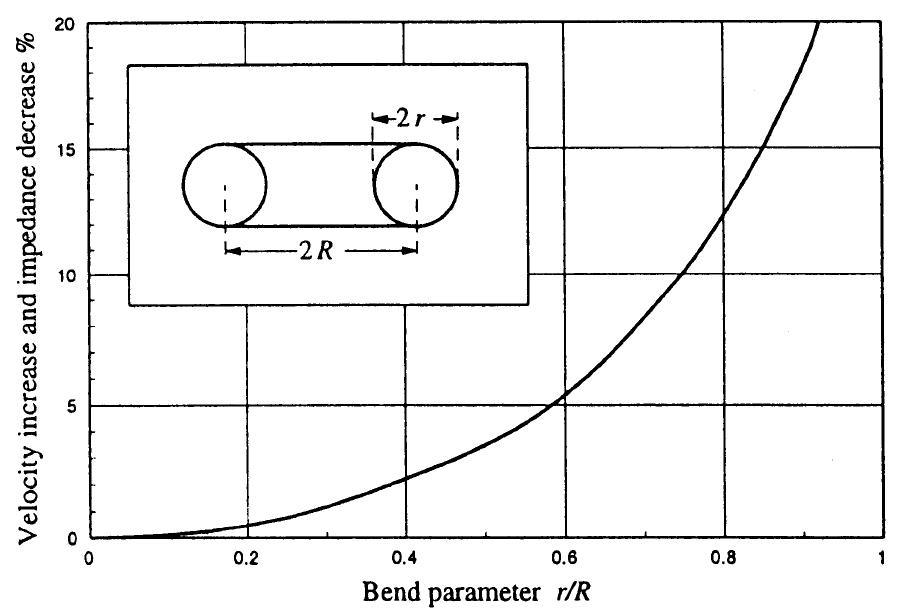
\includegraphics[width=0.7\linewidth]{00_Images/06_chapter/img445.jpg}
    \caption{Effect of horn curvature on wave speed and impedance versus \( B = r/R \)}
    \label{fig:curved_horn_effects}
\end{figure}

For a curved horn, the relative increase in phase velocity and the relative decrease in duct impedance can be expressed as
\[
\frac{\delta v}{c} = -\frac{\delta Z}{Z_{0}} = \left(\frac{2I}{\pi B}\right)^{1/2} - 1
\]
with
\[
I = \int_{0}^{\pi/2} \cos\theta \ln\left(\frac{1 + B\cos\theta}{1 - B\cos\theta}\right)d\theta
\]
As shown by the plot of \( \delta v \) and \( -\delta Z \) versus \( B \), the effect is negligible for small curvature but grows rapidly as \( B \) increases.

\section{Analysis in the Time Domain}

The analysis in the time domain is useful to describe the transient behavior of a wind instrument. Starting from the input impedance \( Z(\omega) \), its inverse Fourier transform defines the Green function \( G(t) \), which relates the acoustic volume flow \( U(t) \) to the pressure \( p(t) \) through convolution
\[
p(t) = \int_{-\infty}^{t} G(t-t')U(t')dt' = G(t)\star U(t)
\]
A direct evaluation is often inconvenient because \( G(t) \) may have a large time support. 

\subsection{Reflection Function Formulation}

Define the plane-wave reflection function at the instrument input as
\[
r(\omega) = \frac{Z(\omega)-Z_{0}}{Z(\omega)+Z_{0}}
\]
where \( Z_{0} \) is the characteristic impedance of the cylindrical reference duct. This implies
\[
Z(\omega) = Z_{0} + Z_{0}r(\omega) + r(\omega)Z(\omega)
\]
Taking the inverse Fourier transform yields
\[
G(t) = Z_{0}\delta(t) + Z_{0}\delta(t)\star r(t) + r(t)\star G(t)
\]
and substituting into the pressure relation gives
\[
p(t) = Z_{0}U(t) + Z_{0}r(t)\star U(t) + r(t)\star p(t)
\]
Equivalently,
\[
p(t) = Z_{0}U(t) + \int_{0}^{\infty} r(t')\left[Z_{0}U(t-t') + p(t-t')\right]dt'
\]

\subsection{Practical Approximation}

The pressure \( p(t) \) is zero for times shorter than the wave-return transit time \( \tau \) along the cylindrical part of the bore. Moreover, \( p(t) \) is smaller than \( G(t) \) because the returning waves are partially absorbed by the matching input termination. These observations justify neglecting the term involving \( p(t-t') \) inside the integral, which makes the computation feasible in practice. 

\section{Coupling Between Pipe and Mechanical Oscillator}

The goal of this section is to illustrate how the coupling between an air cavity and an elastic structure modifies the dynamics of the structure. This situation is encountered in most stringed instruments and also in many percussion instruments. The structure is modeled as a single-degree-of-freedom oscillator, while the cavity is assumed one-dimensional. 

\subsection{Governing Equations}

We consider a pipe of cross section \( S \) and length \( L \), excited at \( x=0 \) by a mechanical oscillator of mass \( M \), resonance angular frequency \( \omega_{0} \), and reduced damping \( \zeta_{0} \). The excitation force is \( f(t) \). Visco-thermal losses in the pipe are neglected. The pipe is terminated at \( x=L \) by a mechanical impedance \( Z_{L} \). The coupled system can be written as
\[
\frac{1}{c^{2}}\frac{\partial^{2}p}{\partial t^{2}}=\frac{\partial^{2}p}{\partial x^{2}}
\]
\[
\rho\frac{\partial u}{\partial t}=-\frac{\partial p}{\partial x}
\]
\[
M\left(\ddot{\xi}+2\zeta_{0}\omega_{0}\dot{\xi}+\omega_{0}^{2}\xi\right)=-Sp(x=0,t)+f(t)
\]
\[
u(0,t)=\dot{\xi}(t)
\]
The termination condition at \( x=L \) is
\[
P(L,j\omega)=Z_{L}(j\omega)V(L,j\omega)
\]
where \( P \) and \( V \) denote Fourier transforms of pressure and particle velocity. 

\subsection{Pipe Input Impedance seen by the Oscillator}

Using continuity at \( x=0 \) and the transfer impedance of a finite duct, the pressure at the coupling point can be written as
\[
P(x=0,j\omega)=\rho c u(0,j\omega)z(j\omega)=j\omega\rho c \Xi(j\omega)z(j\omega)
\]
where \( \Xi \) is the Fourier transform of \( \xi \) and
\[
z(j\omega)=\frac{\tanh(j\omega L/c)+z_{L}}{1+z_{L}\tanh(j\omega L/c)}
\]
with the normalized load
\[
z_{L}=\frac{Z_{L}}{\rho c S}
\]
Substituting into the oscillator equation yields
\[
\left(-\omega^{2}+2j\omega\zeta_{0}\omega_{0}+\omega_{0}^{2}\right)\Xi(j\omega)=\frac{F(j\omega)}{M}-j\omega\frac{\rho c S}{M}\Xi(j\omega)z(j\omega)
\]
so that
\[
\Xi(j\omega)=\frac{F(j\omega)}{M}\frac{1}{-\omega^{2}+2j\omega\omega_{0}\left[\zeta_{0}+\zeta_{a}z(j\omega)\right]+\omega_{0}^{2}}
\]
where \( \zeta_{a} \) is defined by
\[
2\zeta_{a}\omega_{0}=\frac{\rho c S}{M}
\]
The coupling therefore modifies the poles of the mechanical response through the frequency dependence of \( z(j\omega) \), and in particular affects the eigenfrequencies of the combined system. 

\subsection{Particular Cases}

\paragraph{Matched termination} If \( Z_{L}=\rho c S \), then \( z_{L}=1 \) and there is no reflection. In this case \( z(j\omega)=1 \), which corresponds also to an infinite pipe. The coupling increases the effective damping of the oscillator, since the term \( \zeta_{a} \) adds to \( \zeta_{0} \).

\paragraph{Closed pipe, lumped limit} If the pipe is closed at \( x=L \), then \( Z_{L}\to\infty \) and
\[
z(j\omega)=\frac{1}{\tanh(j\omega L/c)}
\]
If the pipe is short enough that \( \tanh(j\omega L/c)\approx j\omega L/c \), then
\[
z(j\omega)\approx\frac{c}{j\omega L}
\]
and the displacement becomes
\[
\Xi(j\omega)=\frac{F(j\omega)}{M}\frac{1}{-\omega^{2}+2j\omega\zeta_{0}\omega_{0}+\omega_{0}^{2}+\frac{2\omega_{0}\zeta_{a}c}{L}}
\]
In this regime the air in the pipe behaves as an added stiffness
\[
K_{a}=\frac{2\omega_{0}M\zeta_{a}c}{L}=\frac{\rho c^{2}S^{2}}{V}
\]
with \( V=SL \). The effect is relevant only if \( K_{a} \) is comparable to the mechanical stiffness \( M\omega_{0}^{2} \). 

\paragraph{Open pipe, lumped limit} If the pipe is open at \( x=L \) and radiation is neglected, \( Z_{L}=0 \) and
\[
z(j\omega)=\tanh(j\omega L/c)
\]
For a short pipe at low frequency, \( \tanh(j\omega L/c)\approx j\omega L/c \), hence
\[
\Xi(j\omega)=\frac{F(j\omega)}{M}\frac{1}{-\omega^{2}+2j\omega\zeta_{0}\omega_{0}+\omega_{0}^{2}-\frac{2\omega^{2}\omega_{0}\zeta_{a}L}{c}}
\]
The pipe acts as an added mass, which in this approximation is
\[
M_{a}=\frac{2M\omega_{0}\zeta_{a}L}{c}=\rho V
\]
with \( V=SL \).
